    
		 \section{Determinante}
		 Die Determinante ist eine Kennzahl dafür, ob eine \textbf{quadratische} Matrix singulär oder regulär ist. \\
		 \\
		  \begin{tabular}{ll}
		    regulär: & $\det(A) \neq 0$ \\
		    singulär: & $ \det(A) = 0$ \\
		  \end{tabular}
		    
		    \subsection{Notation}
		     $A = \begin{bmatrix}
		    			a & b & c \\
		    			d & e & f \\
		    			g & h & i 
		    		\end{bmatrix}$  \qquad  $\det(A) = \begin{vmatrix}
		    			a & b & c \\
		    			d & e & f \\
		    			g & h & i 
		    			\end{vmatrix}$ \\
		    
		    
		    \subsection{Definierende Eigenschaften der Determinante}
		    \begin{tabular}{ll}
		    1. & Wenn eine Zeile mit einem Faktor $\lambda$ multipliziert wird, \\ 
		    & so wird auch $\det(A)$ mit $\lambda$ multipliziert \\
		    2. & $\det(A)$ ändert nicht bei blauen Operationen \\
		    3. & $\det(E)$ = 1 \\
		    4. & Wenn A singulär ist ($\det(A) = 0$) dann ist auch $A^t$ singulär\\
		    & $\det(A^t) = 0$ \\
		    \end{tabular}

			\subsection{Geometrische Interpretation der Determinante}
			\subsubsection{Fläche}
			Orientierter Flächeninhalt des Parallelogramms aufgespannt durch die Vektoren $\vec{a}$ und $\vec{b}$ \\
			\\
 			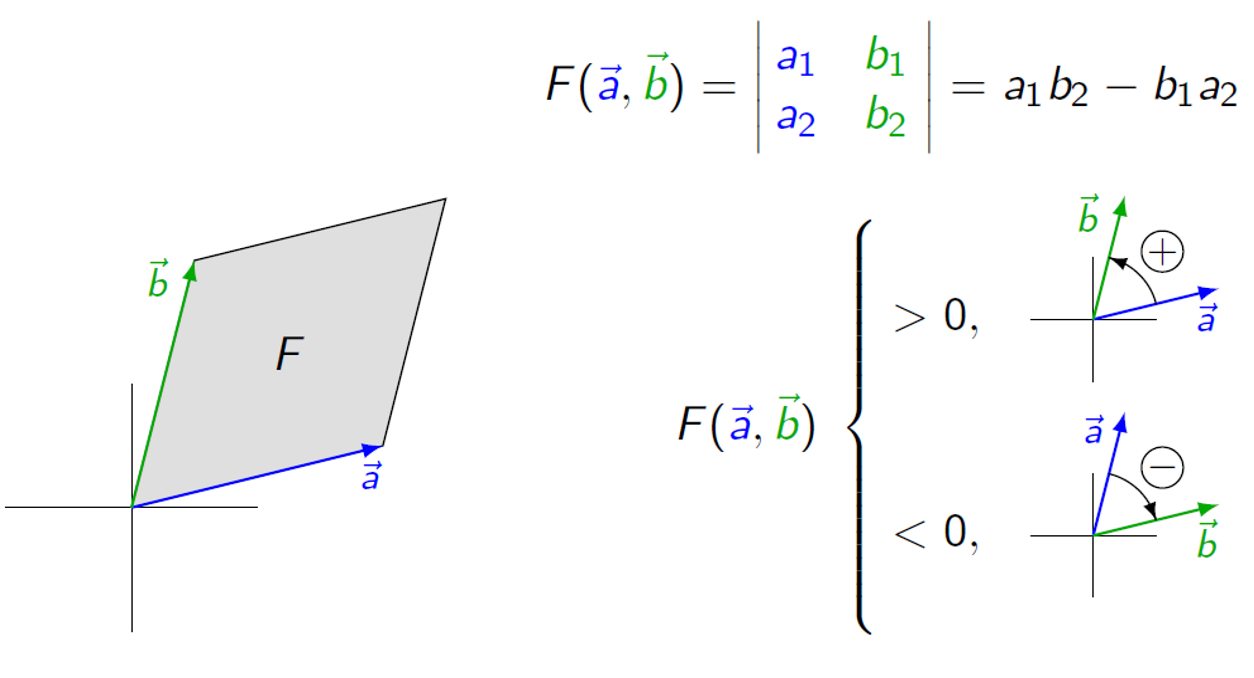
\includegraphics[width=0.7\linewidth]{Bilder/flaeche-det} \\
			
			
			\subsubsection{Volumen}				    
		    Orientiertes Volumen eines Parallelepipeds (Spat) aufgespannt durch die Vektoren $\vec{a}$, $\vec{b}$ und $\vec{c}$ \\
			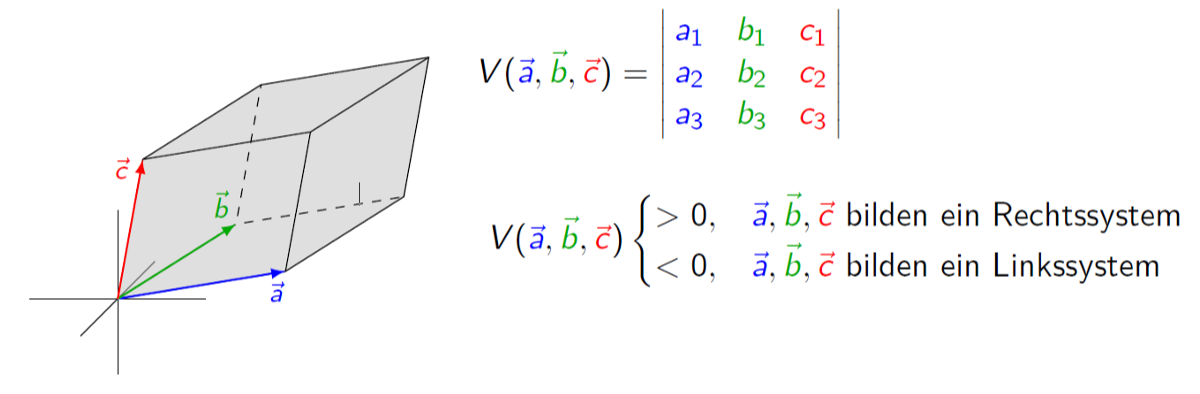
\includegraphics[width=0.9\linewidth]{Bilder/volumen-det} \\
				
				
				
			\hfill\null	
			\columnbreak	
			
			
							
								
			\subsection{Allgemeine Berechnung der Determinante}
			Die Determinante kann mithilfe des Gauss-Algorithmus berechnet werden. Die Determinante ist das \textbf{Produkt} aller Pivot-Elemente. \\
			(Rückwärts-Einsetzen beim Gauss-Verfahren nicht nötig) \\
			\\
			 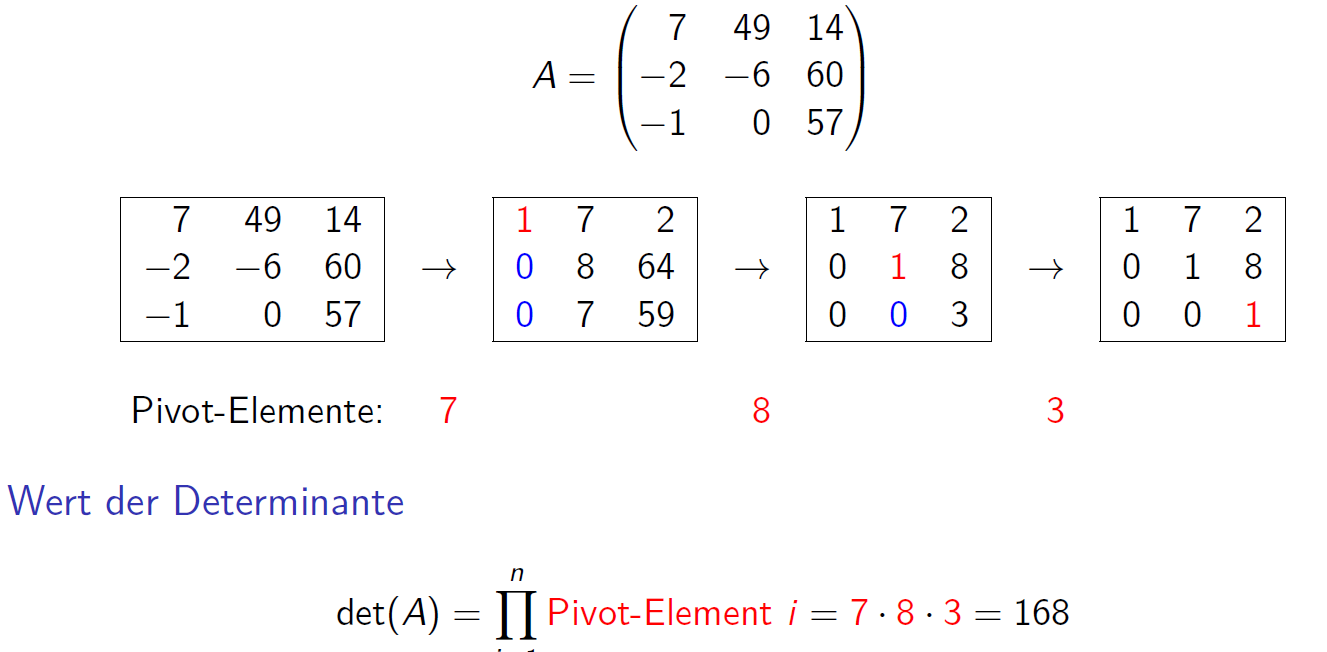
\includegraphics[width=0.8\linewidth]{Bilder/wert-determinante}
			 

		    \subsection{Sarrus}
		    \subsubsection{2 x 2 Matrix}
		    $\det(A) \quad= 	\begin{vmatrix}
		    				a & b \\
		    				c & d
		    				\end{vmatrix}$ =  $ad - bc$ \\
		    	
		    	\subsubsection{3 x 3 Matrix}
		    $\det(A) \quad= 	\begin{vmatrix}
		    					a & b &c \\
		    					d & e & f\\
		    					g & h & i
		    				\end{vmatrix}$ =  $aei + bfg + cdh - ceg - afh - bdi$ \\
		    				
		    				
		    \subsection{Rechenregeln für die Determinante}
			\begin{tabular}{ll}
			1. & Enthält A eine Nullzeile/Nullspalte, dann gilt $\det(A) = 0$ \\
		    2. & Sind zwei Zeilen/Spalten der Matrix A gleich, gilt $\det(A) = 0$ \\
		    3. &  Vertauscht man in der Matrix A zwei Zeilen/Spalten, \\
		    &  so ändert das Vorzeichen von $\det(A)$ \\
		    4. & $\det(E) = 1$ \\
		    5. & Die Determinante ist eine lineare Funktion der Zeilen/Spalten \\
		    \\
			\end{tabular}
		    
		    \begin{tabular}{ll}
		    Produktformel: &$\det(A \cdot B) = \det(A) \cdot \det(B)$ \\
		    \\
		    Determinante der Inversen: & $\det(A^{-1}) = \frac{1}{\det(A)}$ \\
		    \\
		    Transponierte Matrix: & $\det(A) = \det(A^T)$ \\
		    \end{tabular}
		    
		    
		    \subsection{Entwicklungssatz}
			
		    \begin{tabular}{ll}
			1. & Zeile oder Spalte mit meisten Nullen auswählen \\
			2. & Element herausschreiben \textbf{(Vorzeichenmatrix beachten!)} \\
			& herausgenommene Elemente, welche 0 sind fallen weg! \\
			3. & Zeile und Spalte von gewähltem Element wegdenken\\
			4. & Rest (Minor) als Determinante mit herausgenommenem \\
			& Element multiplizieren \\
			5. & Schritte 2-4 wiederholen, bis ganze Zeile/Spalte bearbeitet ist \\
			6. & Wenn noch keine 3x3 Determinanten; Schritte 1-5 wiederholen \\
			7. & Wenn 3x3 Determinanten erreicht sind, mit Sarrus-Formel \\
			& Minor-Determinanten konkret ausrechnen	\\	    		
		    \end{tabular}

			
		    \textbf{Vorzeichenmatrix} \\
		    
		    \begin{tabular}{| c | c | c | c |}
		    \hline
		    + & - & + & - \\
		    \hline
		    - & + & - & + \\
		    \hline
		    + & - & + & - \\
		    \hline
		    - & + & - & + \\
		    \hline
		    \end{tabular}
					    
		    \subsubsection{Beispiel Entwicklungssatz}
		    Berechnung der Determinante von Matrix $A$ \\
		    $A = \begin{pmatrix}
		    		4 & 0 & 7 & 0 \\
		    		5 & 8 & 5 & 1 \\
		    		4 & 7 & 4 & 1 \\
		    		8 & 8 & 10 & 1 \\
		    		\end{pmatrix}$ \\
		    		
		    	\vspace{0.3cm}
			
			$\begin{vmatrix}
		    	\color{blue}4 & \color{blue}0 & \color{blue}7 & \color{blue}0 \\
		    	5 & 8 & 5 & 1 \\
		    	4 & 7 & 4 & 1 \\
		    	8 & 8 & 10 & 1 
		    	\end{vmatrix}  =  4 	\begin{vmatrix}
		    						 8 & 5 & 1 \\ 7 & 4 & 1 \\ 8 									& 10 & 1 
								\end{vmatrix} + 7 												\begin{vmatrix}
								5 & 8 & 1 \\ 4 & 7 & 1 \\ 8 & 								8 & 1 
								\end{vmatrix}$ \quad $\rightarrow$ Sarrus \\						 		    
		    
			\subsubsection{Beispiel Inverse Matrix mittels Entwicklungssatz}
			
			$A = \begin{pmatrix}
		    		-1 & \color{blue}-3 & \color{orange}1 \\
		    		\color{green}3 & 3 & \color{red}-2  \\
		    		\color{teal}2 & \color{violet}1 & -3  \\
		    		\end{pmatrix}$  \quad  \begin{tabular}{ll}
		    		1. & det(A) berechnen \\
		    		2. & Minoren gemäss Entwicklungssatz \\
		    		& in $A^{-1}$ schreiben \\
		    		& \textbf{Farben beachten!} \\
		    		3.& Minoren mit Sarrus berechnen \\
		    		\\
					\end{tabular}						

			$A^{-1} = \frac{1}{\det(A)} \begin{pmatrix}
			\begin{vmatrix}	3 & -2 \\ 1 & -3 \end{vmatrix} & \textcolor{green}{- \begin{vmatrix}	-3 & 1 \\ 1 & -3 \end{vmatrix}} & \textcolor{teal}{\begin{vmatrix}	-3 & 1 \\ 3 & -2 \end{vmatrix}} \\
			\\
			\textcolor{blue}{- \begin{vmatrix}	3 & -2 \\ 2 & -3 \end{vmatrix}} & \begin{vmatrix}	-1 & 1 \\ 2 & -3 \end{vmatrix} & 	\textcolor{violet}{- \begin{vmatrix}	-1 & 1 \\ 3 & -2 \end{vmatrix}} \\
			\\
			\textcolor{orange}{\begin{vmatrix}	3 & 3 \\ 2 & 1 \end{vmatrix}} & \textcolor{red}{- \begin{vmatrix}	-1 & -3 \\ 2 & 1 \end{vmatrix}} & \begin{vmatrix}	-1 & -3 \\ 3 & 3 \end{vmatrix} 
									\end{pmatrix}$ \\ \\
				$\rightarrow$ Sarrus-Formel anwenden \\
										
		    
		    \subsection{Cramersche Regel}
			Mit der Cramerschen Regel können ebenfalls Gleichungssysteme von Typ $A \cdot x = b$ gelöst werden. \\
			Jede Unbekannte x wird durch Determinanten berechnet. \\
			\\
			$\rightarrow$ Es müssen n-1 Determinanten berechnet werden!	 \\
			
			\vfill\null
			\columnbreak
			
			
			
			
			\subsubsection{Beispiel Cramersche Regel}
			$A = \begin{pmatrix}
				-1 & -3 & 0 \\
				2 & 3 & -2 \\
				2 & 1 & -3
				\end{pmatrix}$ \qquad $b = \begin{pmatrix}											\color{blue}-7 \\ \color{blue}2 \\ \color{blue}-5	
											\end{pmatrix}$ \\
				\\		
				\\ $x_1 = \frac{\begin{vmatrix}
							\color{blue}-7 & -3 & 0 \\
							\color{blue}2 & 3 & -2 \\
							\color{blue}-5 & 1 & -3 \\
							\end{vmatrix}}{\det(A)} = 1$ \qquad  $x_2 = \frac{\begin{vmatrix}
							-1 & \color{blue}-7 & 0 \\
							2 & \color{blue}2 & -2 \\
							2 & \color{blue}-5 & -3 \\
							\end{vmatrix}}{\det(A)} = 2$ \\
							
							\vspace{0.2cm}
				$x_3 = \frac{\begin{vmatrix}
							-1 & -3 & \color{blue}-7 \\
							2 & 3 & \color{blue}2 \\
							2 & 1 & \color{blue}-5 \\
							\end{vmatrix}}{\det(A)} = 3$ \\			
		    
		    
			\subsection{Matritzengruppen}	
			 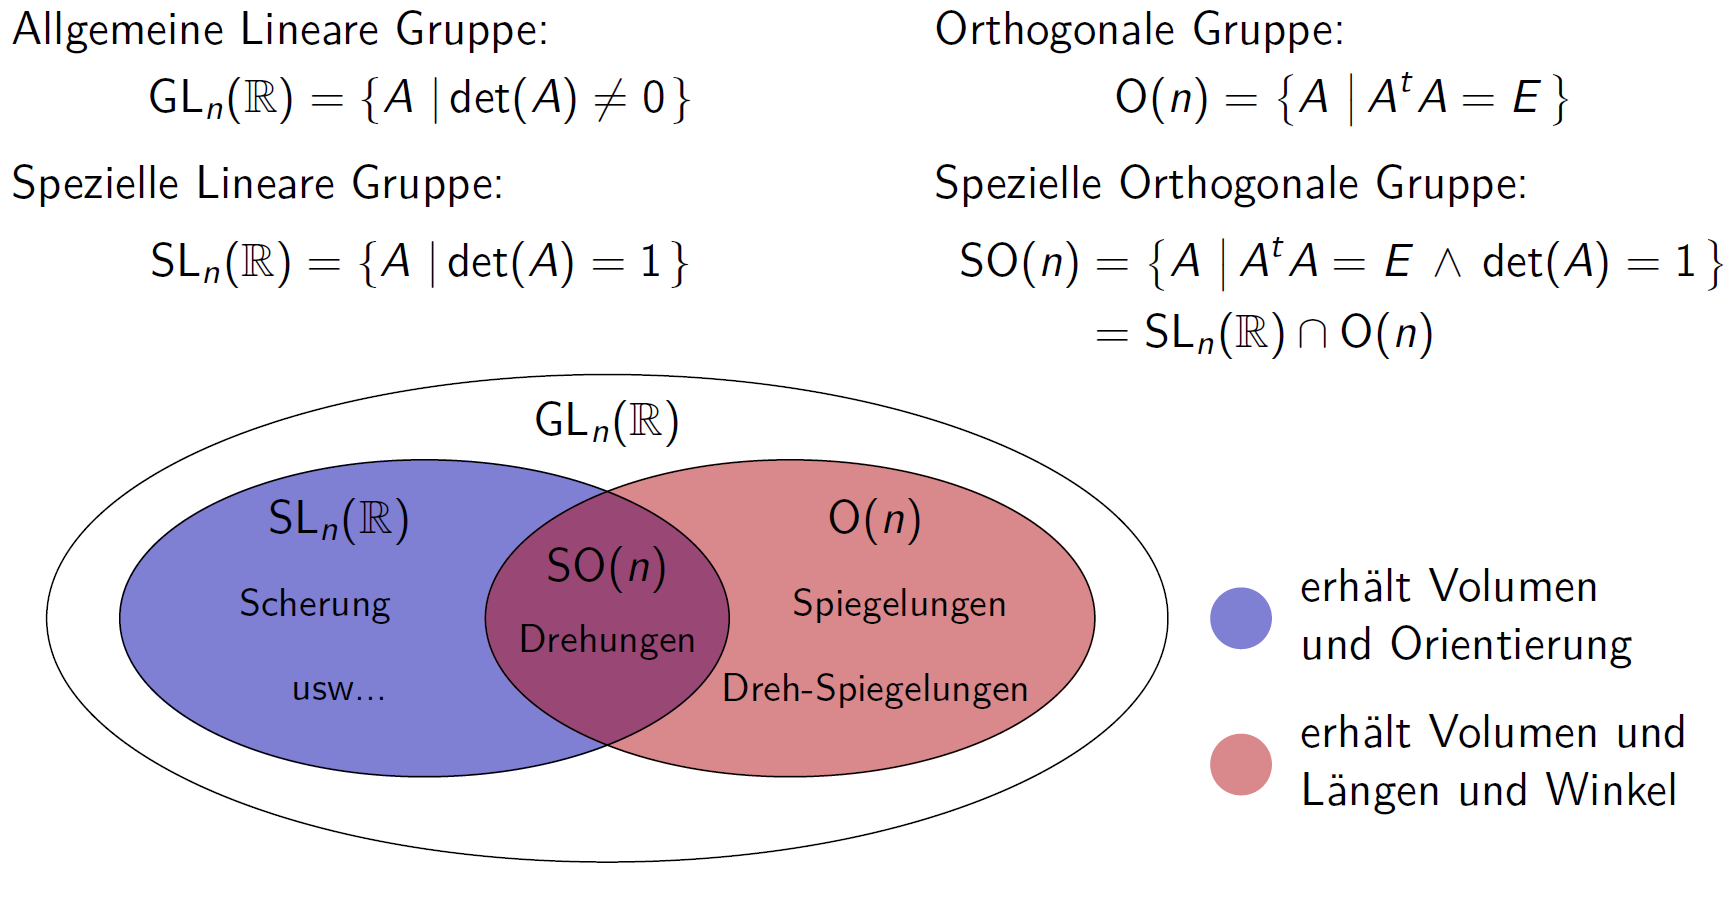
\includegraphics[width=0.8\linewidth]{Bilder/matritzengruppen} \\
		    